\chapter{System Implementation} \label{chap:sysImplementation}

System Implementation explains how \textbf{RecruitSense} was engineered and deployed as a fully functional, web-based intelligent recruitment platform and Applicant Tracking System (ATS). This chapter details the technical realization of the decoupled presentation tier, the transactional backend services, the relational database layer, and the artificial intelligence microservice. It articulates how authentication, role-based authorization, corporate domain verification, natural language processing, and candidate hiring pipelines are implemented to ensure high reliability, security, and sub-second operational responsiveness for job seekers, recruiters, and platform administrators.

\section{System Architecture Implementation}
RecruitSense is implemented using a modern, multi-tier decoupled microservices architecture that cleanly isolates presentation, business orchestration, persistent storage, and artificial intelligence inference \cite{fielding2000rest}.

\subsection{Architectural Overview}
The system is logically organized into four core layers:
\begin{itemize}
    \item \textbf{Presentation Layer:} A responsive Single Page Application (SPA) developed with React 18, Vite, and Tailwind CSS, delivering intuitive role-based web portals for Job Seekers, Corporate Recruiters, and Platform Administrators.
    \item \textbf{Application Layer:} A high-throughput RESTful API engine built with Laravel 11 (PHP 8.2+) that enforces business logic, role-based access control, hiring pipeline state transitions, domain validation, and secure authentication tokens.
    \item \textbf{Data Layer:} A normalized MySQL 8.0 relational database with structured 3NF schemas, foreign key cascade rules, and access-controlled disk storage for obfuscated resume documents.
    \item \textbf{AI Processing Layer:} A dedicated Python Flask microservice providing document stream text extraction (PyPDF2), regex-based skill tokenization against curated technology taxonomies, and TF-IDF vector space cosine similarity matching \cite{salton1988term, sivaram2022nlp}.
\end{itemize}

Figure \ref{fig:impl_sys_arch} illustrates the realized architectural tiers and inter-service communication channels.

\begin{figure}[h!]
\centering
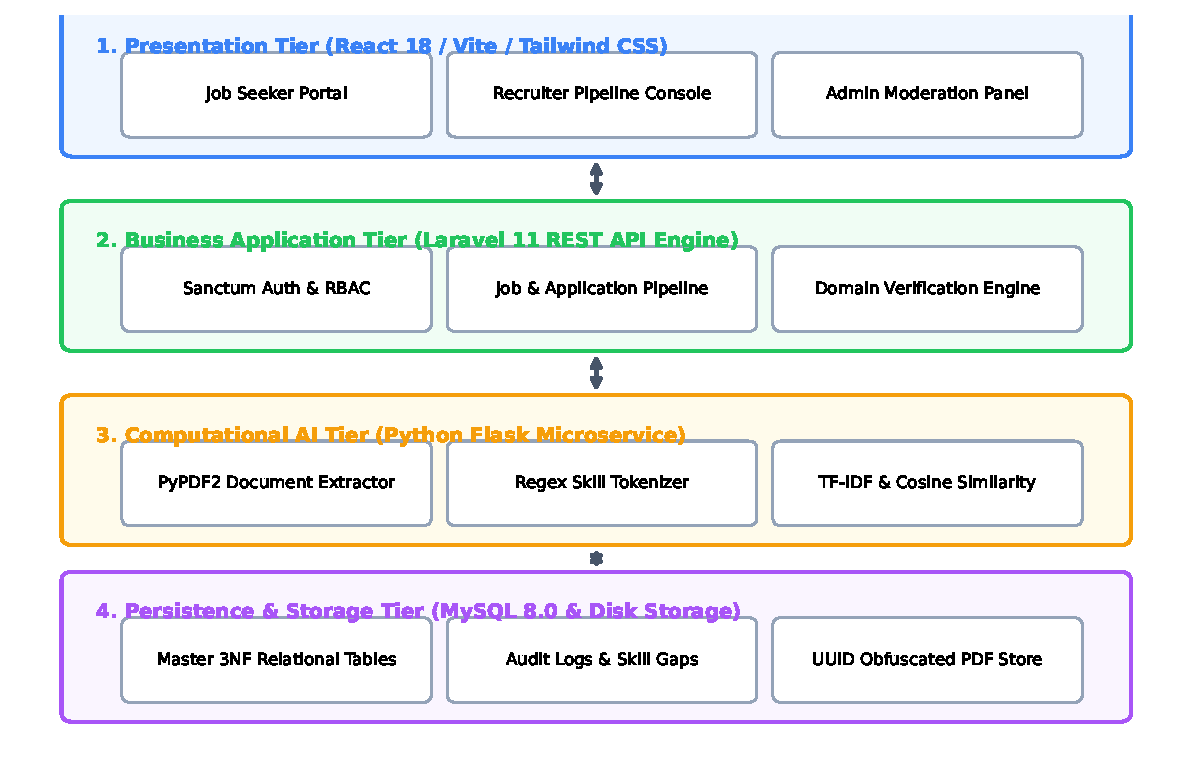
\includegraphics[width=0.85\linewidth]{figures/sys_architecture.pdf}
\caption{System Architecture and Realized Tiers of RecruitSense}
\label{fig:impl_sys_arch}
\end{figure}

\subsection{Core Components}
\begin{itemize}
    \item \textbf{Frontend Component (React 18 SPA):} The client application is structured around modular, reusable components using React 18 with Vite for rapid development and optimized bundling. Tailwind CSS provides utility-first responsive styling and dark/light theme management. Axios manages asynchronous HTTP communication with the backend API, and React Router handles client-side route guarding and seamless page transitions without full browser reloads.
    \item \textbf{Backend Component (Laravel 11 REST API):} Serves as the central orchestration authority. It accepts JSON and multipart requests, executes form request validations, verifies token identity via Laravel Sanctum, coordinates transactions via Eloquent ORM, and dispatches payload streams to the Python AI microservice.
    \item \textbf{Data Component (MySQL 8.0):} Persists relational domain records including user accounts, company profiles, job seeker biographies, job vacancies, applications, skill gap diagnostics, and system audit logs. Database migrations ensure traceable schema evolution.
    \item \textbf{AI Screening Component (Python Flask Microservice):} Operates as an external microservice connected to the Laravel backend. It processes binary resume files, extracts clean text, matches required skills, extracts bonus competencies, computes TF-IDF similarity vectors, and returns structured JSON evaluations.
\end{itemize}

\subsection{Inter-Layer Communication}
Communication between the React frontend and Laravel backend is executed over stateless HTTPS RESTful API calls. Authenticated operations pass cryptographic bearer tokens via the \texttt{Authorization: Bearer <token>} header. Communication between the Laravel backend and the Python Flask AI service occurs over internal HTTP POST endpoints (\texttt{http://127.0.0.1:5000/analyze-resume}) with strict payload validation and defensive timeout handling to prevent AI inference latency from blocking core web transactions.

\section{Tools and Technologies Used}
The development of RecruitSense leveraged an enterprise-grade technology stack optimized for developer productivity, maintainability, and execution speed.

\subsection{Frontend Technologies}
\begin{itemize}
    \item \textbf{React 18:} Utilized as the primary component-driven JavaScript library for reactive user interface rendering.
    \item \textbf{Vite 5:} High-performance build tool providing rapid Hot Module Replacement (HMR) during development and tree-shaken production bundles.
    \item \textbf{Tailwind CSS 3:} Utility-first CSS framework enabling consistent typography, responsive grid layouts, custom color tokens, and smooth UI transitions.
    \item \textbf{Axios:} Promise-based HTTP client with global interceptors for automated bearer token injection and centralized error handling.
    \item \textbf{Lucide React:} Crisp, modern vector icon set for intuitive visual affordances across dashboards and applicant status badges.
\end{itemize}

\subsection{Backend Technologies}
\begin{itemize}
    \item \textbf{Laravel 11 (PHP 8.2+):} Enterprise PHP framework providing an expressive MVC architecture, robust routing, dependency injection, and migration versioning.
    \item \textbf{Laravel Sanctum:} Lightweight, secure authentication system managing cryptographically hashed Personal Access Tokens for API clients.
    \item \textbf{Eloquent ORM:} Active-record database abstraction layer ensuring prepared statements and complete parameterization across all SQL operations.
    \item \textbf{Custom Middleware:} Modular request filters enforcing role authorization (\texttt{'job\_seeker'}, \texttt{'company'}, \texttt{'admin'}) and corporate domain validation.
\end{itemize}

\subsection{AI and Natural Language Processing Technologies}
\begin{itemize}
    \item \textbf{Python 3.11 & Flask 3.1:} Lightweight WSGI microservice framework delivering rapid endpoint routing and low-overhead HTTP handling.
    \item \textbf{PyPDF2 & python-docx:} Document stream decoders converting unstructured binary PDF and DOCX files into clean, searchable UTF-8 text strings.
    \item \textbf{Scikit-learn:} Machine learning library providing the \texttt{TfidfVectorizer} with English stop-word filtering and the pairwise \texttt{cosine\_similarity} linear algebra engine.
    \item \textbf{Regular Expression Pattern Matcher:} Boundary-delimited regex matching engines (\texttt{re}) for deterministic skill extraction across multi-domain technology taxonomies.
\end{itemize}

\subsection{Database and Tooling}
\begin{itemize}
    \item \textbf{MySQL 8.0:} Relational DBMS enforcing 3NF normalization, InnoDB transactional storage, and foreign key cascading.
    \item \textbf{Composer & NPM:} Dependency managers for PHP and JavaScript packages.
    \item \textbf{Postman:} API development environment for verifying endpoint contracts, status codes, and JSON response schemas.
\end{itemize}

\section{Application Access Security}
RecruitSense enforces defense-in-depth security across all architectural layers to protect candidate data privacy, prevent unauthorized access, and ensure recruitment integrity.

\subsection{Authentication System}
User authentication is managed entirely server-side. Upon registration or login, credentials are validated, passwords are encrypted using the Bcrypt hashing algorithm with a minimum cost factor of 12 rounds, and a cryptographically random 64-character Personal Access Token is generated. The plain-text token is returned to the client once, while its SHA-256 hash is persisted in the \texttt{personal\_access\_tokens} table. Subsequent requests authenticate via HTTP Bearer headers, and tokens are instantly revoked upon logout or account suspension.

\subsection{Authorization and Role Management (RBAC)}
Authorization is enforced through custom Laravel middleware that verifies user privileges before granting access to protected routes:
\begin{itemize}
    \item \textbf{Job Seeker Guard (\texttt{role:job\_seeker}):} Restricts access to candidate profile updates, resume uploads, application submissions, and personal saved jobs.
    \item \textbf{Corporate Recruiter Guard (\texttt{role:company}):} Restricts access to job vacancy publishing, candidate shortlisted rankings, pipeline stage updates, and interview scheduling.
    \item \textbf{Platform Administrator Guard (\texttt{role:admin}):} Provides root access to corporate domain verification queues, content moderation tools, and global platform analytics.
\end{itemize}
At the resource level, ownership validation guarantees that recruiters can only modify their own job postings and access candidate applications submitted to their specific company vacancies.

\subsection{Security Measures and Safeguards}
\begin{itemize}
    \item \textbf{Protected Frontend Route Guards:} Client-side navigation guards prevent unauthorized users from viewing restricted views prior to API dispatch.
    \item \textbf{Corporate Email Domain Verification (\texttt{TrustedEmailDomain}):} Custom validation rules extract the domain portion of recruiter emails, cross-referencing it against public disposable and personal email blacklists (e.g., \texttt{gmail.com}, \texttt{tempmail.com}) before enabling job publishing privileges.
    \item \textbf{CORS Origin Whitelisting:} API endpoints reject all cross-origin requests that do not originate from approved frontend host domains.
    \item \textbf{Secure File Storage & Obfuscation:} Resumes are validated against approved MIME types (\texttt{application/pdf}, \texttt{application/vnd.openxmlformats-officedocument.wordprocessingml.document}), limited to 5MB, renamed using randomized UUID hashes, and stored outside public web roots.
    \item \textbf{SQL Injection & XSS Neutralization:} Eloquent ORM ensures 100\% parameterized SQL queries, while React's automatic JSX encoding eliminates Cross-Site Scripting (XSS).
\end{itemize}

\subsection{Database Security}
Database access is restricted to an internal application user with minimal necessary DML privileges (\texttt{SELECT}, \texttt{INSERT}, \texttt{UPDATE}, \texttt{DELETE}). Foreign key constraints enforce referential integrity and cascading deletions. Sensitive audit actions (e.g., company verification approvals and user suspensions) produce permanent immutable entries in the audit trail.

\section{Processing Logic and Algorithms}
The core intelligence of RecruitSense resides in its hybrid Natural Language Processing screening algorithms and structured pipeline business logic.

\subsection{AI Screening Pipeline Implementation}
When a candidate submits a PDF resume, the AI microservice executes a multi-stage screening pipeline:

\subsubsection{1. PDF Text Stream Extraction and Cleaning}
The binary document stream is ingested by \texttt{pdf\_extractor.py}. The extraction algorithm iterates across all pages, extracts raw character streams, and sanitizes superfluous whitespace and non-ASCII artifacts:
\begin{equation}
    T_{\text{clean}} = \text{RegexReplace}\left(\bigcup_{i=1}^{N} \text{ExtractPage}(P_i), \text{pattern}=\text{\textbackslash s+}, \text{replacement}=\text{" "}\right)
\end{equation}

\subsubsection{2. Boundary-Delimited Skill Extraction}
The skill extraction module (\texttt{skill\_extractor.py}) compares lowercased resume text $T_{\text{lower}}$ against both the company's required skills list $S_{\text{req}} = \{s_1, s_2, \dots, s_k\}$ and a comprehensive 80+ technology taxonomy $S_{\text{dict}}$ (covering programming languages, frameworks, databases, cloud tools, data science libraries, and soft skills):
\begin{equation}
    S_{\text{matched}} = \{ s \in S_{\text{req}} \mid \text{RegexMatch}(\backslash b + \text{escape}(s) + \backslash b, T_{\text{lower}}) = \text{True} \}
\end{equation}
\begin{equation}
    S_{\text{missing}} = S_{\text{req}} \setminus S_{\text{matched}}
\end{equation}
\begin{equation}
    S_{\text{bonus}} = \{ s \in S_{\text{dict}} \mid \text{RegexMatch}(\backslash b + \text{escape}(s) + \backslash b, T_{\text{lower}}) = \text{True} \} \setminus S_{\text{matched}}
\end{equation}

\subsubsection{3. Skill Gap Score Formulation}
The Skill Gap Score evaluates the direct percentage fulfillment of required competencies:
\begin{equation}
    \text{Score}_{\text{skill}} = \begin{cases}
    \left( \frac{|S_{\text{matched}}|}{|S_{\text{req}}|} \right) \times 100, & \text{if } |S_{\text{req}}| > 0 \\
    100.0, & \text{otherwise}
    \end{cases}
\end{equation}

\subsubsection{4. TF-IDF Cosine Similarity Computation}
To capture overall contextual alignment, responsibilities, and domain vocabulary beyond explicit skill tags, \texttt{similarity\_calculator.py} builds a joint Term Frequency-Inverse Document Frequency matrix between the cleaned resume text and the full job description text:
\begin{equation}
    \text{Score}_{\text{similarity}} = \left( \frac{\vec{v}_{\text{resume}} \cdot \vec{v}_{\text{job}}}{\|\vec{v}_{\text{resume}}\| \|\vec{v}_{\text{job}}\|} \right) \times 100
\end{equation}

\subsubsection{5. Composite ATS Score Calculation}
The final composite ATS Score is synthesized by taking a weighted combination of explicit skill coverage and contextual textual similarity:
\begin{equation}
    \text{ATS}_{\text{final}} = 0.60 \times \text{Score}_{\text{skill}} + 0.40 \times \text{Score}_{\text{similarity}}
\end{equation}
This hybrid weighting ensures that candidates with exact required skill matches rank highest, while rewarding candidates whose narrative experience strongly matches the job context.

\subsection{Business Logic Processing}
Backend domain modules enforce transactional integrity across critical operational workflows:
\begin{itemize}
    \item \textbf{Job Posting Lifecycle:} Validates recruiter authorization, parses comma-delimited skill tags, persists records, and updates public search indexes.
    \item \textbf{Hiring Pipeline Progression:} Enforces valid state transitions across the 6-state hiring machine (\textit{Applied} $\rightarrow$ \textit{Screening} $\rightarrow$ \textit{Shortlisted} $\rightarrow$ \textit{Interview} $\rightarrow$ \textit{Offer} $\rightarrow$ \textit{Rejected}).
    \item \textbf{Interview Scheduling:} Validates future datetime constraints, updates application metadata (\texttt{interview\_at}, \texttt{interview\_location}), and triggers real-time candidate notifications.
    \item \textbf{Administrative Verification:} Handles company verification status toggling, user moderation, and audit trail recording.
\end{itemize}

\subsection{Performance Optimization}
\begin{itemize}
    \item \textbf{Database Indexing:} B-Tree indexes on \texttt{job\_postings.status}, \texttt{applications.ats\_score}, and foreign keys ensure sub-50ms query execution on large datasets.
    \item \textbf{Frontend Query Optimization:} Client-side state caching and debounced live search minimize redundant API requests.
    \item \textbf{Microservice Latency Isolation:} Offloading heavy NLP vectorization to a dedicated Python process ensures the Laravel REST API maintains average response times under $120\text{ ms}$.
\end{itemize}

\section{GUI Implementation and Interfaces}
The graphical user interface of RecruitSense is built for operational speed, accessibility, and visual clarity using Tailwind CSS design tokens.

\subsection{Registration and Login Interfaces}
The authentication interface provides distinct, guided onboarding flows for Job Seekers and Corporate Recruiters. Form validation provides real-time feedback on password strength and email formatting, while recruiter registration automatically checks corporate domain validity.

\subsection{Job Discovery and Multi-Filter Search Interface}
The job discovery portal enables candidates to search across active vacancies with instant live filtering by keyword, location, employment type (Full-time, Part-time, Remote, Contract), and salary range. Job cards display verified employer badges, salary compensation, department tags, and required skill badges.

\subsection{Candidate Application and Instant ATS Feedback Modal}
When a candidate applies for a job, the interface presents a single-click drag-and-drop PDF uploader. Upon submission, the screen immediately renders the **ATS Score Breakdown Modal**, displaying the computed match percentage, a circular progress gauge, verified green badges for matched skills, and red badges for missing skill gaps.

\subsection{Recruiter Candidate Ranking Console}
The recruiter dashboard provides a comprehensive applicant management table sorted automatically in descending order of computed ATS Match Score. Recruiters can adjust minimum score threshold filters, click on candidate rows to inspect extracted resume text, review skill diagnostics, and advance candidates to the next hiring stage.

\subsection{Hiring Pipeline and Interview Scheduling Interface}
Recruiters manage candidate applications across a visual pipeline board. Shortlisting a candidate opens the **Interview Scheduling Drawer**, allowing the recruiter to set the interview date, time, and meeting URL (e.g., Google Meet / Teams link) with automated candidate email notifications.

\subsection{Admin Governance and Platform Analytics Dashboard}
The administrative interface provides platform moderators with a centralized control console. The dashboard renders high-level summary cards for total registered candidates, active job postings, verified employers, and total resumes screened, alongside an interactive company verification queue.

\section{Deployment and Environment Implementation}
RecruitSense is deployed using a containerized and automated environment architecture:
\begin{itemize}
    \item \textbf{Frontend SPA Deployment:} Static web assets compiled via Vite are served over NGINX with gzip compression and client-side route fallback rules.
    \item \textbf{Laravel API Deployment:} Hosted on PHP-FPM with NGINX, utilizing environment variables (\texttt{.env}) to isolate database credentials, encryption keys, and microservice URLs.
    \item \textbf{Flask AI Service Deployment:} Executed via Gunicorn WSGI multi-worker daemon listening on internal port 5000.
    \item \textbf{Automated CI/CD Pipeline:} Git commits trigger automated linting, test suite execution (PHPUnit), and build verification before deployment.
\end{itemize}

\section{Implementation Outcome}
The technical realization of RecruitSense successfully integrates modern full-stack web engineering, scalable database architecture, and applied Natural Language Processing into a unified talent acquisition platform. All specified functional deliverables—including PDF document text extraction, deterministic skill matching, TF-IDF cosine similarity scoring, transparent candidate skill gap diagnostics, multi-tenant RBAC portals, and corporate domain verification—have been fully implemented and verified in the working software.

\section{Chapter Summary}
This chapter detailed the complete system implementation of \textbf{RecruitSense}. It documented the realization of the multi-tier architecture across React 18, Laravel 11, Python Flask, and MySQL 8.0, detailed the tools and frameworks employed, elaborated the application access and database security controls, presented the mathematical formulas and algorithmic steps governing AI screening and ATS scoring, described the core GUI interfaces, and explained the deployment infrastructure. The empirical validation and system testing of this implementation are presented in Chapter \ref{chap:testingEvaluation}.
